% Questo file conterrà i domini trattati nelle lezioni
\section{Domini non relazionali}

Questa sezione introduce i domini non relazionali, che rappresentano
astrazioni più semplici rispetto ai domini relazionali, in quanto
considerano ogni variabile indipendentemente dalle altre.

\subsection{Dominio dei segni}

Il dominio dei segni è un dominio astratto classico utilizzato per l'analisi
statica di programmi che manipolano numeri interi.
L'obiettivo di questa astrazione è determinare se una variabile assume valori
positivi, negativi o nulli durante l'esecuzione.

\subsubsection{Struttura del reticolo}

Il dominio concreto di riferimento è $\wp(\mathbb{Z})$ (l'insieme delle parti
degli interi).
Il dominio astratto, denotato come $D^\sharp$, è costituito da un insieme
finito di elementi che approssimano gli insiemi di interi in base al loro
segno.

Gli elementi del dominio $D^\sharp$ sono:
\begin{itemize}
    \item $\top$: Rappresenta l'intero insieme $\mathbb{Z}$ (qualsiasi valore
    è possibile, ``non so'').
    \item $(+)$: Rappresenta l'insieme dei numeri strettamente positivi
    $\{z \in \mathbb{Z} \mid z > 0\}$.
    \item $(0)$: Rappresenta l'insieme singoletto $\{0\}$.
    \item $(-)$: Rappresenta l'insieme dei numeri strettamente negativi
    $\{z \in \mathbb{Z} \mid z < 0\}$.
    \item $\bot$: Rappresenta l'insieme vuoto $\emptyset$ (nessun valore
    possibile, codice irraggiungibile).
\end{itemize}

Questi elementi formano un reticolo completo (\Cref{def:complete_lattice}).
La relazione d'ordine parziale (\Cref{def:partial_order}) $\sqsubseteq$
riflette l'inclusione insiemistica delle concretizzazioni.
Graficamente, il reticolo è piatto (flat) nella parte centrale, con $\bot$
come elemento minimo e $\top$ come elemento massimo.

\begin{figure}[H]
    \centering
    \begin{tikzpicture}
        \node (top) at (0,1.5) {$\top$};
        \node (p) at (-1.5,0) {$(+)$};
        \node (z) at (0,0) {$(0)$};
        \node (n) at (1.5,0) {$(-)$};
        \node (bot) at (0,-1.5) {$\bot$};

        \draw (bot) -- (p);
        \draw (bot) -- (z);
        \draw (bot) -- (n);
        \draw (p) -- (top);
        \draw (z) -- (top);
        \draw (n) -- (top);
    \end{tikzpicture}
    \caption{Reticolo del dominio dei segni.}
    \label{fig:sign_lattice}
\end{figure}

\subsubsection{Funzione di astrazione e concretizzazione}

La relazione tra il dominio concreto e dominio astratto è definita tramite una
connessione di Galois (\Cref{def:galois_connection}) $(\alpha, \gamma)$:
\begin{itemize}
    \item \textbf{Funzione di astrazione} $\alpha: \wp(\mathbb{Z}) \to D^\sharp$:
    dato un insieme di interi $S \subseteq \mathbb{Z}$, $\alpha(S)$ restituisce
    il più piccolo elemento astratto che contiene $S$.
    \item \textbf{Funzione di concretizzazione} $\gamma: D^\sharp \to \wp(\mathbb{Z})$:
    dato un elemento astratto $d \in D^\sharp$, $\gamma(d)$ restituisce
    l'insieme concreto di interi rappresentato da $d$.
\end{itemize}

La funzione $\alpha$ è definita come:
\[
\alpha(S) =
\begin{cases}
    \bot & \text{se } S = \emptyset \\
    (+) & \text{se } S \subseteq \{z \in \mathbb{Z} \mid z > 0\} \\
    (0) & \text{se } S = \{0\} \\
    (-) & \text{se } S \subseteq \{z \in \mathbb{Z} \mid z < 0\} \\
    \top & \text{altrimenti}
\end{cases}
\]
La funzione $\gamma$ è definita come:
\[
\gamma(d) =
\begin{cases}
    \emptyset & \text{se } d = \bot \\
    \{z \in \mathbb{Z} \mid z > 0\} & \text{se } d = (+) \\
    \{0\} & \text{se } d = (0) \\
    \{z \in \mathbb{Z} \mid z < 0\} & \text{se } d = (-) \\
    \mathbb{Z} & \text{se } d = \top
\end{cases}
\]

\subsubsection{Operazioni astratte}
Le operazioni aritmetiche concrete (come $+$, $-$, $\times$, $\div$) devono
essere ridefinite sul dominio astratto per preservare la correttezza
(soundness).
\begin{nota}{Logica delle operazioni astratte}{abstract_operations_logic}
La logica generale per definire le operazioni astratte sul dominio dei segni
segue il principio della ``regola dei segni'':
\begin{itemize}
    \item La somma di due numeri positivi è positiva.
    \item La somma di due numeri negativi è negativa.
    \item La somma di un numero positivo e uno negativo può essere positiva,
    negativa o zero, a seconda dei valori specifici.
    \item La somma di zero con qualsiasi numero restituisce quel numero.
\end{itemize}

Questa logica si estende alle altre operazioni aritmetiche, tenendo conto
delle regole matematiche fondamentali.
\end{nota}

\paragraph{Operazione di somma}
L'operazione di somma astratta $\oplus: D^\sharp \times D^\sharp \to D^\sharp$
è definita come:
\[
d_1 \oplus d_2 =
\begin{cases}
    \bot & \text{se } d_1 = \bot \text{ o } d_2 = \bot \\
    (+) & \text{se } d_1 = (+) \text{ e } d_2 = (+) \\
    (+) & \text{se } d_1 = (+) \text{ e } d_2 = (0) \\
    (+) & \text{se } d_1 = (0) \text{ e } d_2 = (+) \\
    (-) & \text{se } d_1 = (-) \text{ e } d_2 = (-) \\
    (-) & \text{se } d_1 = (-) \text{ e } d_2 = (0) \\
    (-) & \text{se } d_1 = (0) \text{ e } d_2 = (-) \\
    (0) & \text{se } d_1 = (0) \text{ e } d_2 = (0) \\
    \top & \text{altrimenti}
\end{cases}
\]

\paragraph{Operazione di moltiplicazione}
L'operazione di moltiplicazione astratta $\otimes: D^\sharp \times D^\sharp \to D^\sharp$
è definita come:
\[
d_1 \otimes d_2 =
\begin{cases}
    \bot & \text{se } d_1 = \bot \text{ o } d_2 = \bot \\
    (+) & \text{se } (d_1 = (+) \text{ e } d_2 = (+)) \text{ o } (d_1 = (-) \text{ e } d_2 = (-)) \\
    (-) & \text{se } (d_1 = (+) \text{ e } d_2 = (-)) \text{ o } (d_1 = (-) \text{ e } d_2 = (+)) \\
    (0) & \text{se } d_1 = (0) \text{ o } d_2 = (0) \\
    \top & \text{altrimenti}
\end{cases}
\]

\paragraph{Operazione di negazione}
L'operazione di negazione astratta $\text{neg}: D^\sharp \to D^\sharp$
è definita come:
\[
\text{neg}(d) =
\begin{cases}
    \bot & \text{se } d = \bot \\
    (-) & \text{se } d = (+) \\
    (0) & \text{se } d = (0) \\
    (+) & \text{se } d = (-) \\
    \top & \text{se } d = \top
\end{cases}
\]

\paragraph{Operazione di sottrazione}
L'operazione di sottrazione astratta $\ominus: D^\sharp \times D^\sharp \to D^\sharp$
è definita come:
\[
d_1 \ominus d_2 = d_1 \oplus \text{neg}(d_2)
\]

\paragraph{Operazione di divisione}
L'operazione di divisione astratta $\oslash: D^\sharp \times D^\sharp \to D^\sharp$
deve gestire il caso speciale della divisione per zero:
\[
d_1 \oslash d_2 =
\begin{cases}
    \bot & \text{se } d_1 = \bot \text{ o } d_2 = \bot \\
    \top & \text{se } d_2 = (0) \text{ o } d_2 = \top \\
    (+) & \text{se } (d_1 = (+) \text{ e } d_2 = (+)) \text{ o } (d_1 = (-) \text{ e } d_2 = (-)) \\
    (-) & \text{se } (d_1 = (+) \text{ e } d_2 = (-)) \text{ o } (d_1 = (-) \text{ e } d_2 = (+)) \\
    (0) & \text{se } d_1 = (0) \\
    \top & \text{altrimenti}
\end{cases}
\]

\begin{nota}{Rappresentazione delle operazioni come tabella}{operations_table}
Le operazioni astratte possono essere rappresentate in forma tabellare per
facilitare la consultazione e l'implementazione.

\begin{center}
\begin{tabular}{c|ccccc}
$+^\sharp$ & $\bot$ & $(-)$ & $(0)$ & $(+)$ & $\top$ \\
\hline
$\bot$ & $\bot$ & $\bot$ & $\bot$ & $\bot$ & $\bot$ \\
$(-)$ & $\bot$ & $(-)$ & $(-)$ & $\top$ & $\top$ \\
$(0)$ & $\bot$ & $(-)$ & $(0)$ & $(+)$ & $\top$ \\
$(+)$ & $\bot$ & $\top$ & $(+)$ & $(+)$ & $\top$ \\
$\top$ & $\bot$ & $\top$ & $\top$ & $\top$ & $\top$ \\
\end{tabular}
\end{center}

\end{nota}

\begin{nota}{Perdita di precisione}{loss_of_precision}
È importante notare come alcune operazioni astratte possano portare a una
perdita di precisione nell'analisi:
\begin{itemize}
\item La somma di due numeri positivi è sicuramente positiva: $(+) +^\sharp (+) = (+)$.
\item La somma di un positivo e un negativo non ha un segno determinato nel
dominio astratto, risultando in $\top$ (``non so'').
\end{itemize}
\end{nota}

\subsection{Dominio dei valori costanti}

Il dominio dei valori costanti (\Cref{def:constant_propagation}) è un
dominio astratto non relazionale utilizzato per determinare se una
variabile assume un unico valore determinato durante tutte le possibili
esecuzioni di un programma in un dato punto.

\subsubsection{Struttura del reticolo}
Il dominio astratto, denotato come $\mathcal{B}^\sharp_{CP}$,
è costruito estendendo l'insieme dei valori concreti (es. interi
$\mathbb{Z}$) con due elementi speciali:
\begin{itemize}
    \item $\bot$: Rappresenta l'insieme vuoto (codice irraggiungibile o
    variabile non inizializzata).
    \item $\top$: Rappresenta l'incertezza (``non so''), ovvero la
    variabile può assumere più valori distinti.
\end{itemize}

\begin{esempio}{Dominio dei valori costanti su $\mathbb{Z}$}{constant_propagation}
Il reticolo del dominio dei valori costanti su $\mathbb{Z}$ è definito come
\[
CP = \langle \mathbb{Z} \cup \{\bot\} \cup \{\top\}, \sqsubseteq, \bot, \top, \sqcup, \sqcap \rangle
\]
e rappresentato graficamente come segue:
\begin{figure}[H]
    \centering
    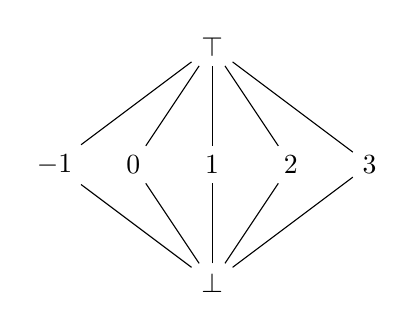
\begin{tikzpicture}
        \node (top) at (0,1.5) {$\top$};
        \node (n1) at (-2,0) {$-1$};
        \node (n0) at (-1,0) {$0$};
        \node (p1) at (0,0) {$1$};
        \node (p2) at (1,0) {$2$};
        \node (p3) at (2,0) {$3$};
        \node (bot) at (0,-1.5) {$\bot$};

        \draw (bot) -- (n1);
        \draw (bot) -- (n0);
        \draw (bot) -- (p1);
        \draw (bot) -- (p2);
        \draw (bot) -- (p3);
        \draw (n1) -- (top);
        \draw (n0) -- (top);
        \draw (p1) -- (top);
        \draw (p2) -- (top);
        \draw (p3) -- (top);
    \end{tikzpicture}
\end{figure}
\end{esempio}

Questo reticolo è definito come un reticolo piatto (flat lattice) ma di
larghezza infinita.
Tutti i valori costanti $c \in \mathbb{Z}$ sono incomparabili tra loro, ma
vale sempre $\bot \sqsubset c \sqsubset \top$.

\subsubsection{Operazioni astratte}
Le operazioni fondamentali per l'analisi sono il \textit{Join}
($\sqcup$, unione astratta) e le operazioni aritmetiche astratte.


\paragraph{Join ($\sqcup$)}
L'operazione di unione è definita come segue:
\begin{equation}
    x \sqcup y = \begin{cases} 
    x & \text{se } x = y \\
    x & \text{se } y = \bot \\
    y & \text{se } x = \bot \\
    \top & \text{altrimenti (es. } x,y \in \mathbb{Z}, x \neq y \text{)}
    \end{cases}
\end{equation}
Questa definizione implica che se due flussi di controllo portano valori costanti diversi per la stessa variabile (es. $3$ e $4$), l'informazione viene persa e il risultato diventa $\top$.

\paragraph{Aritmetica Astratta}
Le operazioni (es. $+^\sharp, -^\sharp$) sono definite applicando l'operazione concreta se entrambi gli operandi sono costanti. Se uno degli operandi è $\top$, il risultato è generalmente $\top$.

\begin{nota}{Eccezione nelle operazioni aritmetiche}{arithmetic_exception}
 Anche se un operando è sconosciuto ($\top$), la moltiplicazione per $0$
 restituisce sempre $0$, preservando precisione:
\begin{equation}
    0 \times^\sharp \top = 0
\end{equation}
\end{nota}

\subsubsection{Connessione di Galois}
La relazione tra il dominio concreto $\wp(\mathbb{Z})$ e dominio astratto $CP$
è definita tramite una connessione di Galois (\Cref{def:galois_connection})
$(\alpha, \gamma)$:
\begin{itemize}
    \item \textbf{Funzione di astrazione} $\alpha: \wp(\mathbb{Z}) \to D^\sharp$:
    dato un insieme di interi $S \subseteq \wp(\mathbb{Z})$, $\alpha(S)$ è
    definito come:
    \[
    \alpha(S) =
    \begin{cases}
        \bot & \text{se } S = \emptyset \\
        c & \text{se } S = \{c\} \\
        \top & \text{se } |S| > 1
    \end{cases}
    \]
    \item \textbf{Funzione di concretizzazione} $\gamma: D^\sharp \to \wp(\mathbb{Z})$:
    dato un elemento astratto $d \in D^\sharp$, $\gamma(d)$ è definita come:
    \[
    \gamma(a) =
    \begin{cases}
        \emptyset & \text{se } a = \bot \\
        \{c\} & \text{se } a = c \in \mathbb{Z} \\
        \mathbb{Z} & \text{se } a = \top
    \end{cases}
    \]
\end{itemize}

\begin{nota}{Limitazioni del dominio dei valori costanti}{constant_propagation_limitations}
Le analisi basate sul dominio dei valori costanti sono limitate dal fatto che
non sono analisi distributive (\Cref{def:distributivity}).
Ciò significa che astrarre il risultato delle operazioni sui singoli rami e
poi unire i risultati è più preciso che unire gli stati astratti prima di
eseguire l'operazione.
\end{nota}

\paragraph{Convergenza}
Poiché il reticolo ha altezza finita (massimo 3 livelli: $\bot \to c \to
\top$), non esistono catene ascendenti infinite.
Di conseguenza, l'operatore di widening (\Cref{def:widening_operator}) può
coincidere semplicemente con l'operatore di join ($\sqcup$), garantendo
comunque la terminazione dell'analisi in tempo finito senza necessità
di soglie o euristiche complesse.